\documentclass[]{article}
\usepackage{amssymb}
\usepackage{amsmath}
\usepackage[utf8]{inputenc}
\usepackage{graphicx}
\usepackage{booktabs}
\usepackage{listings}
\usepackage{color}
\usepackage{tabularx}
\usepackage{hyperref}

\definecolor{dkgreen}{rgb}{0,0.6,0}
\definecolor{gray}{rgb}{0.5,0.5,0.5}
\definecolor{mauve}{rgb}{0.58,0,0.82}

\lstset{frame=tb,
	%language=C++,
	aboveskip=3mm,
	belowskip=3mm,
	showstringspaces=false,
	columns=flexible,
	basicstyle={\small\ttfamily},
	numbers=none,
	numberstyle=\tiny\color{gray},
	keywordstyle=\color{blue},
	commentstyle=\color{dkgreen},
	stringstyle=\color{mauve},
	breaklines=false,
	breakatwhitespace=true,
	tabsize=2
}

\title{FYS4150 Project 3:\\Celestial Mechanics with Numerical Methods}
\author{Olav Fønstelien}

\begin{document}
\maketitle

\begin{abstract}
%The abstract gives the reader a quick overview of what has been done and the most important results. Try to be to the point and state your main findings. It could be structured as follows 
% - Short introduction to topic and why its important 
% - Introduce a challenge or unresolved issue with the topic (that you will try to solve) 
% - What have you done to solve this 
% - Main Results 
% - The implications


\end{abstract}


\section{Introduction} \label{intro}
%When you write the introduction you could focus on the following aspects
% - Motivate the reader, the first part of the introduction gives always a motivation and tries to give the overarching ideas
For all its beauty, the limits of differential calculus quickly becomes apparent when it comes to the study of planetary movements. The classic $n$-body problem for describing the movement of bodies in interacting gravitational fields can be perfectly accounted for with closed form for $n=2$, but problems arise already at $n=3$. Hence the need for numerical methods, and in this report we will develop an $n$-body \textit{solver} based on the \textit{Velocity Verlet} algorithm \cite{fys4150-notes}. 

% - What I have done
% - The structure of the report, how it is organized etc
Lets first revisit some of the basics of celestial mechanics, which will serve as a mathematical background for our development of the algorithms.





\section{Background: Celestial Mechanics} \label{celestial-mechanics}
It was \textit{Johannes Kepler} (1571-1630) who first described the planets' orbits correctly. By observation he found that all planets move in elliptic orbits with the sun at one of the two foci; and that the square of their periods $T$ are directly proportional to the cube of their semi-major axis $a$ \cite{hibbeler2001} (Kepler's first and third laws, respectively). Perfect harmony prevailed, it seemed:
\begin{equation}
	T^2 \propto a^3.
\end{equation}
Later, \textit{Isaac Newton} (1642-1727) would describe with his gravitational law the mutual attractive force $F_G$ between two bodies of mass $M, m$ at distance $r$ apart as
\begin{equation} \label{newton-grav}
	F_G = \frac{GMm}{r^2},
\end{equation}
where $G$ is the gravitational constant. Further, as a result of Newton's second law, the centripetal force acting on a body with mass $m$ moving along a circular path with radius $r$ at angular velocity $\omega$ is given by
\begin{equation}
	F_C = mr\omega^2.
\end{equation}
Kepler, having died 12 years before Newton's birth, would have been astonished when he discovered that when combining these laws, his own would have been confirmed. For the simple case of a circular orbit, with the Sun's mass $M$, the planet mass $m$, and the angular velocity $\omega = 2\pi/T$, we get by equating $F_G$ and $F_C$ that
\begin{equation} \label{r3-T2}
	mr\bigg(\frac{2\pi}{T}\bigg)^2 = \frac{GMm}{r^2} \Rightarrow \frac{r^3}{T^2} = \frac{GM}{4\pi^2}.
\end{equation}

An important result of this combination of Newton's gravitational and second laws is that they postulate the conditions for closed elliptic orbits. Following \cite{hibbeler2001}, a planetary orbit's \textit{eccentricity} is given by
\begin{equation}
	e = \frac{r_0 v_0^2}{GM} - 1,
\end{equation}
where $r_0$ is the planet's distance from the Sun at any of the orbit's vertices, and $v_0$ is the velocity at that point. Calculating $e$ we get the trajectories:
\begin{equation}
\begin{aligned}
	e < 1 \quad &: \quad \text{closed elliptic} \\
	e \ge 1 \quad &: \quad \text{parabolic/hyperbolic trajectory}.
\end{aligned}
\end{equation}
The special case $e=0$ gives a circular orbit, and for the cases $e \ge 1$, the planet escapes into space, never to return. This is easily seen by reminding ourselves that the sum of the planet's kinetic energy, $E_K=\frac{1}{2}mv^2$, and potential energy, $E_P=-GMm/r$, is preserved during flight, such that
\begin{equation}
E = E_K + E_P = \frac{1}{2}mv^2 - GMm/r = const.
\end{equation}
Now, if the sum at the vertex is zero or positive we have that
\begin{equation}
	\frac{1}{2}mv_0^2 \ge \frac{GMm}{r_0} \Rightarrow \frac{r_0v_0^2}{GM} \ge 2 \Rightarrow e \ge 1,
\end{equation}
and since $E_K \ge E_P$, the planet will escape. For the circular orbit, we recall from Equation (\ref{r3-T2}) that $F_G = F_C$, such that
\begin{equation} \label{e=0}
	\frac{mv_0^2}{r_0} = \frac{GMm}{r_0^2} \Rightarrow \frac{r_0 v_0^2}{GM} = 1 \Rightarrow e = 0.
\end{equation}
We note that in a circular orbit, $E_K = \frac{1}{2} E_P$.

The last of Kepler's observations was that the planets move in their orbits such that the line joining it to the sun sweeps over equal areas in equal intervals of time, whatever the line's length. Again, see \cite{hibbeler2001}. This observation of constant \textit{areal velocity}, called Kepler's second law, can be written
\begin{equation}
	\frac{dA}{dt} = \frac{1}{2} r^2 \frac{d\theta}{dt} = const. \quad.
\end{equation}
It would also be explained as a consequence of Newton's discoveries. The \textit{angular momentum} of a body with mass $m$ moving at velocity $\mathbf{v}$ at distance $\mathbf{r}$ from a fixed point $O$ is defined as $\mathbf{L}_O = \mathbf{r} \times m\mathbf{v}$. Now, with $\mathbf{r}$ and $\mathbf{v}$ at an angle $\phi$ to each other, $|\mathbf{r} \times \mathbf{v}| = rv \sin \phi$; and the component of $\mathbf{v}$ perpendicular to $\mathbf{r}$ is the body's velocity on a circular path about $O$, so $v \sin \phi = r \frac{d\theta}{dt}$. Bringing this all together, we get that Kepler's second law foresaw the conservation of angular momentum:
\begin{equation}
	\mathbf{L}_O = L_O\mathbf{e} = (mrv \sin \phi )\mathbf{e} = mr^2 \frac{d\theta}{dt} \mathbf{e} = 2m \frac{dA}{dt} \mathbf{e} = \text{\textit{const. vector}} \quad,
\end{equation}
where $\mathbf{e}$ is a unit vector.

\section{Numerical Methods for Celestial Mechanics} \label{methods}
% - Describe the methods and algorithms
% - You need to explain how you implemented the methods and also say something about the structure of your algorithm and present some parts of your code
% - You should plug in some calculations to demonstrate your code, such as selected runs used to validate and verify your results. The latter is extremely important!! A reader needs to understand that your code reproduces selected benchmarks and reproduces previous results, either numerical and/or well-known closed form expressions.

We will start with developing a solver for the simplified 2-body problem with a fixed Sun at the center and a planet moving around it. We will use this for proving the correctness our algorithm, as well as studying its efficiency with regards to CPU time and accuracy. Then, we will proceed to solving the general $n$-body problem in an object-oriented manner. At the end of this section, we briefly discuss the inclusion of a general relativistic factor for calculating the slow rotation of the perihelion of Mercury.

\subsection{Sun-Earth System with Fixed Sun} \label{sun-earth}
The location at time $t+h$ of an body moving along a straight line with non-constant velocity $v = v(t)$, is given by the Taylor expansion
\begin{equation}
	x(t+h) = x(t) + hv(t) + O(h^2),
\end{equation}
where $O(h^2)$ is the truncation error. The velocity $v(t+h)$ at the new position $x(t+h)$, is again given by a new Taylor series
\begin{equation}
	v(t+h) = v(t) + h \frac{dv}{dt}(t) + O(h^2) \quad \text{, where} \quad \frac{dv}{dt}(t) = a(t).
\end{equation}
We discretize time in the time interval $[t, t + \Delta t]$ by letting $t_i = t + ih$, where $i \in [0,n]$ and $h = \Delta t/n$. We then get the discrete equations for the body's motion as
\begin{equation}
\begin{aligned}
	x_{i+1} &= x_i + hv_i \\
	v_{i+1} &= v_i + ha_i
\end{aligned} \quad.
\end{equation}


With these equations, called \textit{Euler's forward method}, we can can iteratively calculate the object's movement along the $x$ axis, and expanding to three dimensions yields corresponding equations for movement along the $y$ and $z$ axes. 

To apply Euler's forward method on Newton's gravitational law (\ref{newton-grav}), we must plug in Newton's gravitational law (\ref{newton-grav}) for the acceleration. On vector form and in spherical coordinates the acceleration is given as
\begin{equation} \label{a-spherical}
	\mathbf{a}_i = \frac{GM}{r_i^3} \mathbf{r}_i.
\end{equation}
where $M$ is the mass of the attracting body. In the Solar System it is convenient to refer time, mass and space to the Earth-Sun system. Hence, we will scale away $GM$ from Equation (\ref{a-spherical}) using the relationship we found in Equation (\ref{r3-T2}), namely $GM = 4\pi^2r^3/T^2$, where $M$ is the mass of the Sun, $r = 1$ AU, and $T = 1$ year, such that
\begin{equation} \label{a-spherical}
	GM = 4\pi^2 \quad \text{[AU}^3/\text{yr.}^2\text{].}
\end{equation}


Now, the with cartesian representation of $\mathbf{a}_i$, we get the full set of forward Euler equations in three dimensions for solving the problem of planetary movement about the Sun, where the Sun is kept fixed at the center:
\begin{equation} \label{euler-fwd}
\begin{aligned}
	&x_{i+1} = x_i + hv_{x,i} ,\quad v_{x,i+1} = v_{x,i} - 4\pi^2h\frac{x_i}{r_i^3} ,\\
	&y_{i+1} = y_i + hv_{y,i} ,\quad v_{y,i+1} = v_{y,i} - 4\pi^2h\frac{y_i}{r_i^3} ,\\
	&z_{i+1} = z_i + hv_{z,i} ,\quad v_{z,i+1} = v_{z,i} - 4\pi^2h\frac{z_i}{r_i^3} ,\\
\end{aligned}
\end{equation}
where $r_i = \sqrt{x_i^2 + y_i^2 + z_i^2}$. A framework of the algorithm is given in Listing \ref{lst:euler} below.

\begin{lstlisting}[caption={Euler's Forward algorithm for Sun-Earth system with fixed Sun.},label={lst:euler}] [!ht]
	// Declarations
	n = "number of steps per year"
	y = "years to calculate"
	N = y*n  // total number of steps
	h = 1.0/n  // time step length
	array(3) position = "initial x,y,z"
	array(3) velocity = "initial vx, vy, vz"
	array(3) pos0  // for storing postion after update
	
	// Iterations
	FOR i = 1...N DO
		pos0 = position
		position = position + h*velocity
		r = norm(pos0)
		velocity = velocity - h*4*pi^2/r^3*pos0
	END DO
\end{lstlisting}

A problem with Euler's Forward method, though, is that it does not conserve energy, it is not symplectic \cite{notes-10-02}. This can be shown by evaluating a few iterations. A correction to this energy leak is possible with the small modification $x_{i+1} = x_i + hv_{x,i+1}$, known as the the \textit{Euler-Cromer method}. However, this too has a truncation error $O(h^2)$, which means that it quickly becomes too coarse or inefficient if we want to calculate long time spans with high precision. An alternative method, which is both energy conserving and more precise is the \textit{Velocity Verlet} method. Taking again the Taylor expansion for calculating the movement of a body along a straight line, we have
\begin{equation}
\begin{aligned}
	x(t+h) &= x(t) + hv(t) + \frac{h^2}{2}a(t) + O(h^3) \\
	v(t+h) &= v(t) + ha(t) + \frac{h^2}{2}\frac{d^2v}{dt^2}(t) + O(h^3)
\end{aligned} \quad ,
\end{equation}
where $O(h^3)$ is the truncation error. $\frac{d^2v}{dt^2}(t)$ can itself be found using a Taylor expansion, such that
\begin{equation}
	\frac{d^2v}{dt^2}(t) = \frac{a(t+h) - a(t)}{h} + O(h),
\end{equation}
which, since $h^2O(h)$ yields $O(h^3)$, gives us 
\begin{equation}
\begin{aligned}
	x(t+h) &= x(t) + hv(t) + \frac{h^2}{2}a(t) + O(h^3) \\
	v(t+h) &= v(t) + \frac{h}{2}(a(t+h) + a(t)) + O(h^3)
\end{aligned} \quad .
\end{equation}
We see that we need $a(t+h)$ in order to calculate $v(t+h)$, which may not always be possible. For solving gravitational problems, however, the acceleration is dependent on position only, meaning that if we calculate $x(t+h)$ first, we can obtain $a(t+h)$ and then move on to calculating $v(t+h)$.

Discretizing as we did for Euler's Forward method, we get again the full set of equations for solving the problem of planetary movement about the Sun by the Velocity Verlet method, with the Sun fixed at the center:
\begin{equation} \label{verlet}
\begin{aligned}
	&x_{i+1} = x_i + hv_{x,i} - 2\pi^2h^2\frac{x_i}{r_i^3} , \quad v_{x,i+1} = v_{x,i} - 2\pi^2h \bigg(\frac{x_{i+1}}{r_{i+1}^3} + \frac{x_i}{r_i^3} \bigg) ,\\
	&y_{i+1} = y_i + hv_{y,i}- 2\pi^2h^2\frac{y_i}{r_i^3} , \quad v_{y,i+1} = v_{y,i} - 2\pi^2h \bigg(\frac{y_{i+1}}{r_{i+1}^3} + \frac{y_i}{r_i^3} \bigg) ,\\
	&z_{i+1} = z_i + hv_{x,i}- 2\pi^2h^2\frac{z_i}{r_i^3} , \quad v_{z,i+1} = v_{z,i} - 2\pi^2h \bigg(\frac{z_{i+1}}{r_{i+1}^3} + \frac{z_i}{r_i^3} \bigg) ,\\
\end{aligned}
\end{equation}
where $r_i = \sqrt{x_i^2 + y_i^2 + z_i^2}$. See Listing \ref{lst:verlet-nonOO} below for an algorithm framework.

\begin{lstlisting}[caption={Velocity Verlet algorithm for Sun-Earth system with fixed Sun.},label={lst:verlet-nonOO}] [!ht]
	// Declarations
	n = "number of steps per year"
	y = "years to calculate"
	N = y*n  // total number of steps
	h = 1.0/n  // time step length
	array(3) position = "initial x,y,z"
	array(3) velocity = "initial vx, vy, vz"
	array(3) acceleration
	array(3) acc0  // for storing acceleration after update
	
	// Initializing
	r = norm(position)
	acceleration = -4*pi^2/r^3*position
	
	// Iterations
	FOR i = 1...N DO
		position = position + h*velocity - h^2/2*acceleration
		acc0 = acceleration
		r = norm(pos0)
		acceleration = -4*pi^2/r^3*position
		velocity = velocity - h/2*(acceleration + acc0)
	END DO
\end{lstlisting}

Comparing the Verlocity Verlet method with Euler's Forward method, we see that Euler's is more efficient with regards to FLOPs (FLoting point OPersations) per iteration. Euler needs one multiplication and one addition for each position $x_i, y_i, z_i$; plus two multiplications and one subtraction for each velocity $v_{x,i}, v_{y,i}, v_{z,i}$. 15 FLOPs in total. However, $r_i$ and the factor $r_i^{-3}$ must be calculated once per iteration. This involves square root and floating point divide operations, which are much more expensive than regular FLOPs and are not pipelined properly in the CPU \cite{hager2010introduction}. For Velocity Verlet, total number of FLOPs is $3+4=7$, and even if the method has both $r_i, r_i^{-3}$ and $r_{i+1}, r_{i+1}^{-3}$ terms, we store these between the iterations such that the most expensive operations are done only once, as we saw in Listing \ref{lst:verlet-nonOO}.

CPU time for both Euler Forward and Velocity Verlet has a linear relation to problem size, as we see in Table \ref*{tab:cpu-time}. As expected, Euler is the fastest, but more than what we can explain by the FLOPs ratio between the algorithms. A possible explanation is the square root operations, which are bound to make trouble with pipelining. Another possibility is the use of \lstinline|C++ Armadillo| classes. In these completely CPU bound algorithms, these may cause some of the additional variables in Verlet to be stored outside of CPU register, meaning that they must be loaded from L1 cache.

This speed advantage of Euler relative to Verlet is easily offset when we compare the accuracy between the two. As we see in Figure \ref{fig:verlet-euler}, which shows Earth in a circular orbit around the Sun over 100 years, Velocity Verlet is remarkably stable. Even for $n=100$ iteration steps per year, the accumulated error in the energy balance is on the order of $10^{-8}$. For Euler's Forward, we see a complete breakdown even at $n=1000$, partly stemming from its lower accuracy and partly from its non-symplecticity. 

Figure \ref{fig:verlet-euler} also shows that the 1/2 relationship between kinetic and potential energy is conserved for the Verlet results, in accordance with Equation (\ref{e=0}) for eccentricity $e=0$. We also see that after 100 years, Verlet has lagged about 1/8th of a year for $n=100$, so to get good accuracy for long runs, we should use at least $n=1000$. In the following, we will limit our discussion to Velocity Verlet.

\begin{figure}[!htb]
	\centering
	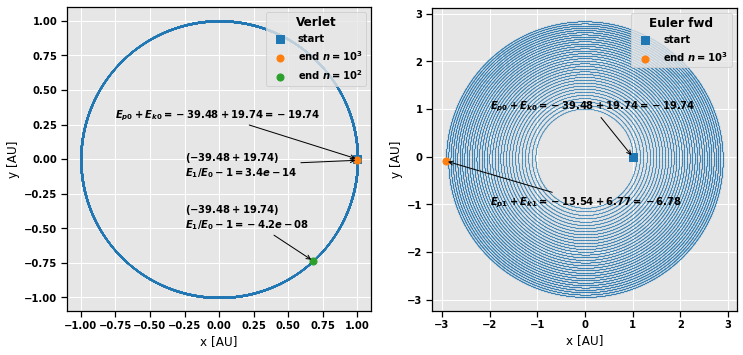
\includegraphics[width=1\linewidth]{verlet-euler.png}
	\caption{Trace of 100 years of the Sun-Earth system with fixed Sun and circular orbit for the Velocity Verlet method to the left and Euler's Forward method to the right. Euler quickly breaks down due to low precision and energy leak, while Verlet has far superior accuracy for a 10th of the iteration steps. Verlet conserves energy with high accuracy even for $n=100$ steps per year, but will lag a bit unless $n$ is selected high enough.}
	\label{fig:verlet-euler}
\end{figure}

\begin{table}[!ht]
	\caption{Averaged CPU times for Euler's Forward and Velocity Verlet algorithms when solving the Sun-Earth system with fixed Sun. Each run is 1 year. As could be expected, as soon as the pipelining reaches its full potential, scaling is perfect. The speed difference between the methods is somewhat surprising, though, since that cannot all be explained by the $7/5=1.4$ FLOPs ratio between them. Both algorithms are CPU-bound. Results were obtained on an Intel i7-8550U CPU, with implementation  in \lstinline|C++| with \lstinline|Armadillo 10.1.0|.}
	\label{tab:cpu-time}
	\begin{center}
		\begin{tabular}{rrrr}
			\toprule
			n &     Euler's Forward [s] &    Velocity Verlet [s] & ratio [\%] \\
			\midrule
			$10^1$ & 2.000e-07 & 1.000e-06 & 500 \\
			$10^2$ & 1.500e-06 & 3.500e-06 & 233 \\
			$10^3$ & 1.450e-05 & 2.980e-05 & 206 \\
			$10^4$ & 1.439e-04 & 2.817e-04 & 196 \\
			$10^5$ & 1.511e-03 & 2.879e-03 & 191 \\
			$10^6$ & 1.543e-02 & 2.699e-02 & 175 \\
			$10^7$ & 1.573e-01 & 2.776e-01 & 176 \\
			$10^8$ & 1.526e+00 & 2.730e+00 & 179 \\
			$10^9$ & 1.530e+01 & 2.735e+01 & 179 \\
			\bottomrule
		\end{tabular}
	\end{center}
\end{table}

\subsection{Solar System} \label{solar-system}
We can extend the Velocity Verlet method in Equation (\ref{verlet}) to the general $n$-body system quite easily. Newton's gravitational law for the acceleration of a body 1 at location $\mathbf{r}_1$ towards a body 2 with mass $m_2$ at location $\mathbf{r}_2$ is given by 
\begin{equation}
	\mathbf{a}_{12} = \frac{Gm_2}{r_{12}^3} \mathbf{r}_{12} \quad , \quad \text{where} \quad \mathbf{r}_{12} = \mathbf{r}_{2} - \mathbf{r}_{1}.
\end{equation}
The total acceleration $\mathbf{a}_{1}$ of body 1 in an $n$-body problem is then simply the sum of the distance vectors to the other bodies, $\mathbf{r}_{1i}$, weighted by their masses $m_i$ over $r_{1i}^3$:
\begin{equation}
	\mathbf{a}_{1} = \sum_{i=2}^{n} \frac{Gm_i}{r_{1i}^3} \mathbf{r}_{1i}.
\end{equation}

As in the Sun-Earth system we then scale away the planet masses and the gravitational constant using $GM = 4 \pi^2$ AU$^3$/yr.$^2$, where $M$ is the Sun's mass, such that
\begin{equation}
	Gm_i = GM \cdot \frac{m_i}{M} = 4\pi^2 \cdot \frac{m_i}{M} = 4\pi^2 \cdot \mu_i.
\end{equation}
For planet $p$ we then get the following set of equations for solving the $n$-body problem using the Velocity Verlet method 
\begin{equation} \label{verlet-n}
\begin{aligned}
	x_{i+1}^{(p)} &= x_i^{(p)} + hv_{x,i}^{(p)} - 2\pi^2h^2 \sum_{\substack{j=1  \\ j \neq p}}^{n} \frac{\mu_j x_i^{(pj)}}{(r_i^{(pj)})^3} \\
	v_{x,i+1}^{(p)} &= v_{x,i}^{(p)} - 2\pi^2h \sum_{\substack{j=1  \\ j \neq p}}^{n} \bigg(\frac{\mu_j x_{i+1}^{(pj)}}{(r_{i+1}^{(pj)})^3} + \frac{\mu_j x_i^{(pj)}}{(r_i^{(pj)})^3} \bigg)	
\end{aligned} \quad ,
\end{equation}
and correspondingly for the $y$ and $z$ axes.

In effect, we need 6 equations per planet. There are 8 planets in the solar system, and counting the Sun and Pluto we have 60 equations to solve. Two strategies which each have their merit are an array-based strategy where we allocate an array of length $n$ for each variable, and keep track of the planets that way, or object orientation, which we will do here.




\section{Results} \label{results}
% - Present your results
% - Give a critical discussion of your work and place it in the correct context.
% - Relate your work to other calculations/studies
% - An eventual reader should be able to reproduce your calculations if she/he wants to do so. All input variables should be properly explained.
% - Make sure that figures and tables should contain enough information in their captions, axis labels etc so that an eventual reader can gain a first impression of your work by studying figures and tables only.


Individual energies have less accuracy than the total.

\section{Discussion and Conclusion} \label{conclusion}
% - State your main findings and interpretations
% - Try as far as possible to present perspectives for future work
% - Try to discuss the pros and cons of the methods and possible improvements

n=100 case has flown only (100-1/8) rounds vs 100 for n=1000, but energy is the same. What does that have to say for the energy?


\clearpage
\bibliographystyle{plain}
\bibliography{project3.bib}
\end{document}
